\section{Before we Begin}\label{before-we-begin}

Our goals are lofty- introducing a new paradigm that combines data
mining with multi-objective optimization. And doing so in such a way
that even novices can understand, use, and adapt these tools for a large
range of new tasks.

But before we can start all that, we have to handle some preliminaries.
All artists, and programmers, should start out as apprentices. If we
were painters and this was Renaissance Italy, us apprentices would spend
decades study the ways of the masters, all the while preparing the
wooden panels for painting; agrinding and mixing pigments; drawing
preliminary sketches, copying paintings, and casting sculptures. It was
a good system that gave us the Michelangelo and Da Vinci who, in turn,
gave us the roof of the Sistine Chapel and the Mona Lisa.

In terms of this book, us apprentices first have to become effective
Python programmers. The rest of this chapter offers:

\begin{itemize}
\itemsep1pt\parskip0pt\parsep0pt
\item
  Some notes on useful web-based programming tools
\item
  Some pointers on learning Python
\item
  Some start-up exercises to test if you have an effective Python
  programming environment.
\end{itemize}

\subsection{Useful On-Line Tools}\label{useful-on-line-tools}

\subsubsection{Stackoverflow}\label{stackoverflow}

To find answers to nearly any question you'll ever want to ask about
Python, go browse:

\begin{lstlisting}
 http://stackoverflow.com/questions/tagged/python
\end{lstlisting}

\subsubsection{Github}\label{github}

All programmers should use off-site backup for their work. All
programmers working in teams should store their code in repositories
that let them fork a branch, work separately, then check back their
changes into the main trunk.

There are many freely-available repository tools. Github is one such
service that supports the \texttt{git} repository tool. Github has some
special advantages:

\begin{itemize}
\itemsep1pt\parskip0pt\parsep0pt
\item
  It is the center of vast social network of programmers;
\item
  Github support serving static web sites straight from your Github
  repo.
\item
  Many other services offer close integration with Github (e.g.~the
  Cloud9 tool discussed below).
\end{itemize}

For more information, go to:

\begin{lstlisting}
 http://github.com
\end{lstlisting}

The good news about Github is that it is very easy to setup and
configure. The bad news is that each Github repository has a 1GB size
limit. But that is certainly enough to get us started.

For Linux/Unix/Mac users, I add the following tip. In each of your
repository directories, add a \texttt{Makefile} with the following
contents.

\begin{lstlisting}
typo:   ready
        @- git status
        @- git commit -am "saving"
        @- git push origin master # update as needed

commit: ready
        @- git status
        @- git commit -a
        @- git push origin master

update: ready
        @- git pull origin master

status: ready
        @- git status

ready:
        @git config --global credential.helper cache
        @git config credential.helper \
             'cache --timeout=3600'

timm:  # <== change to your name
        @git config --global user.name "Tim Menzies"
        @git config --global user.email \
                               tim.menzies@gmail.com
\end{lstlisting}

This \texttt{Makefile} implements some handy shortcuts:

\begin{itemize}
\itemsep1pt\parskip0pt\parsep0pt
\item
  \texttt{make\ typo} is a quick safety save-- do this many times per
  day;
\item
  \texttt{make\ commit} is for making commented commits-- use this to
  comment any improvements .// degradation of functionality.
\item
  \texttt{make\ update} is for grabbing the latest version off the
  server-- do this at least at the start of each day.
\item
  \texttt{make\ status} is for finding files that are not currently
  known to Github.
\item
  \texttt{make\ ready} remembers your Github password for one hour-- use
  this if you use \texttt{make\ typo} a lot and you want to save some
  keystrokes.
\item
  \texttt{make\ timm} should be used if Github complains that it does
  not know who you are. Before running this one, edit this rule to
  include your name and email.
\end{itemize}

Of course, there are 1000 other things you can do with a
\texttt{Makefile}. For example, this book is auto-generated by a
\texttt{Makefile} that automatically extracts comments and code from my
Python source code, then compiles the comments as Markdown, then used
the wonderful \texttt{pandoc} tool to compile the Markdown into Latex,
then converts the Latex to a \texttt{.pdf} file. Which is all
interesting stuff-- but beyond the scope of this book.

\subsubsection{Cloud9}\label{cloud9}

If you do not want to install code locally on your machine, then there
are many readily-available on-line integrated development environments.

For example, to have root access to a fully-configured Unix
installation, you can go to

\begin{lstlisting}
 http://c9.io
\end{lstlisting}

One tip is to host your Cloud9 workspace on Github. As of June 2015, the
procedure for doing that was:

\begin{itemize}
\itemsep1pt\parskip0pt\parsep0pt
\item
  Go to Github and create an empty repository.
\item
  Log in to Cloud9 using your GitHub username (at \texttt{http://c9.io},
  there is a button for that, top right).
\item
  Hit the green \emph{CREATE NEW WORKSPACE} button

  \begin{itemize}
  \itemsep1pt\parskip0pt\parsep0pt
  \item
    Select \emph{Clone from URL};
  \item
    Find \emph{Source URL} and enter in
    \texttt{http://github.com/you/yourRepo}
  \item
    Wait ten seconds for the screen to change.
  \item
    Hit the green \emph{START EDITING} button.
  \end{itemize}
\end{itemize}

This will drop you into the wonderful Cloud9 integrated development
environment. Here, is my editting the above Makefile and some Python
code at Cloud9. I've just run \texttt{make\ typo} so all the changes to
the Python file are now backed up outside of Cloud9, over at
\texttt{Github.com}.

\begin{figure}[htbp]
\centering
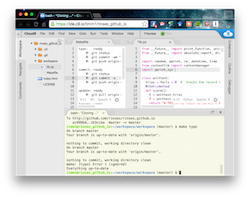
\includegraphics{img/c9400.png}
\caption{The Cloud9 on-line IDE.}
\end{figure}

The good news about Cloud9 is that it is very easy to setup and
configure. The bad news is that each Cloud9 workspace has the same
limits as Github- a 1GB size limit. Also, for CPU-intensive
applications, shared on-line resources like Cloud9 can be a little slow.
That said, for the newbie, Cloud9 is a very useful tool to jump start
the learning process.

\subsection{Python101}\label{python101}

\subsubsection{Why Python?}\label{why-python}

I use Python for two reasons: readability and support. Like any computer
scientist, I yearn to use more powerful languages like LISP or
Javascript or Haskell. That said, it has to be said that good looking
Python is reads pretty good-- no ugly brackets, indentation standards
enforced by the compiler, simple keywords, etc.

Ah, you might reply, but what about other beautiful languages like
CoffeeScipt or Scala or insert yourFavoriteLanguageHere? It turns out
that, at the time of this writing, that there is more tutorial support
for Python that any other language I know. Apart from the many excellent
Python textbooks, the on-line community for Python is very active and
very helpful; e.g.~see stackoverlow.com.

\subsubsection{Installing a ``Good'' Python
Environment}\label{installing-a-good-python-environment}

\subsubsection{Python Standards}\label{python-standards}

This textbook uses Python 2.7 for its code base. Of course, it is
tempting to use Python3 but there are still too many Python packages out
there t

\subsection{Homework}\label{homework}

\subsubsection{Homework1}\label{homework1}

\begin{itemize}
\itemsep1pt\parskip0pt\parsep0pt
\item
  Do: get an account at \texttt{http://github.com}. Hand-in: your Github
  id.
\end{itemize}
